\documentclass[11pt]{article}
\usepackage{geometry}                
\geometry{letterpaper}                   

\usepackage{graphicx}
\usepackage{amssymb}
\usepackage{epstopdf}
\usepackage{natbib}
\usepackage{amssymb, amsmath}
\usepackage{listings}
\graphicspath{ {./images/} }
\DeclareGraphicsRule{.tif}{png}{.png}{`convert #1 `dirname #1`/`basename #1 .tif`.png}

\title{Simulating Vaccinations}
\author{Hannah Niese, Markus Niese, Timo Schönegg}
\date{24.11.2018} 

\begin{document}



\thispagestyle{empty}

\begin{center}

\includegraphics[width=5cm]{ETHlogo.eps}

\bigskip


\bigskip


\bigskip


\LARGE{ 	Lecture with Computer Exercises:\\ }
\LARGE{ Modelling and Simulating Social Systems\\}

\bigskip

\bigskip

\small{Project Report}\\

\bigskip

\bigskip

\bigskip

\bigskip


\begin{tabular}{|c|}
\hline
\\
\textbf{\LARGE{Pertussis resurgence in societies}}\\
\textbf{\LARGE{with high vaccination coverage}}\\
\\
\hline
\end{tabular}
\bigskip

\bigskip

\bigskip

\LARGE{Hannah Niese, Markus Niese \& Timo Schönegg}



\bigskip

\bigskip

\bigskip

\bigskip

\bigskip

\bigskip

\bigskip

\bigskip

\bigskip

\bigskip

\bigskip

\bigskip

\bigskip

Zurich\\
Dec 2018\\

\end{center}



\newpage

%%%%%%%%%%%%%%%%%%%%%%%%%%%%%%%%%%%%%%%%%%%%%%%%%

\newpage
\section*{Agreement for free-download}
\bigskip


\bigskip


\large We hereby agree to make our source code for this project freely available for download from the web pages of COSS. Furthermore, we assure that all source code is written by ourselves and is not violating any copyright restrictions.

\begin{center}

\bigskip


\bigskip


\begin{tabular}{@{}p{0.5cm}@{}p{5.5cm}@{}p{5.5cm}@{}p{5.5cm}@{}p{1cm}}
\begin{minipage}{1cm}

\end{minipage}
&
\begin{minipage}{5cm}
\vspace{2mm} \large Hannah Niese

 \vspace{\baselineskip}

\end{minipage}
&
\begin{minipage}{5cm}

\large Markus Niese

\end{minipage}
&
\begin{minipage}{5cm}

\large Timo Schönegg

\end{minipage}
&
\begin{minipage}{1cm}

\end{minipage}

\end{tabular}


\end{center}
\newpage

%%%%%%%%%%%%%%%%%%%%%%%%%%%%%%%%%%%%%%%



% IMPORTANT
% you MUST include the ETH declaration of originality here; it is available for download on the course website or at http://www.ethz.ch/faculty/exams/plagiarism/index_EN; it can be printed as pdf and should be filled out in handwriting


%%%%%%%%%% Table of content %%%%%%%%%%%%%%%%%

\tableofcontents

\newpage

%%%%%%%%%%%%%%%%%%%%%%%%%%%%%%%%%%%%%%%



\section{Abstract}
The first objective of this paper is to model find which level of immunisation is required to eradicate Pertussis in a society. We simulated the effects of various initial vaccination rates and draw a comparison to theoretical models, and observe the stability of our results. 
The second objective is to find out under wich circumstances Pertussis outbreaks occur, in particular in societies with high vaccination coverage. We find that a lack of  

\section{Individual contributions}

\section{Introduction and Motivations}

Vaccines are without doubt one of the greatest advances in medicine, whose widespread use has lead to the eradication or restriction of some of the deadliest diseases, including smallpox, polio and measles. Every vaccination carries a small risk of side effects. According to the WHO, severe adverse events are extremely rare for most vaccines (for the Hepatitis B vaccine only one in a million is affected) or not yet clinically proven like in the case of Hepatitis A.\footnote{WHO (2018-10-06), $http://www.who.int/vaccine_safety/initiative/tools/vaccinfosheets/en/$}  However, contested medical papers and rumours have led to a reluctance to vaccinate in parts of the society.

\vspace{14px}

We modelled the specific case of Pertussis or Whooping cough, as there have been several incidents where a rising number of infections have been observed despite relatively high vaccination rates. One of these cases is the Netherlands, where, despite a coverage rate of 95\% several cases of Pertussis have been registered. One of the reasons is waning immunisation and the lack of people getting vaccinated. Even though these cases might be few, the survival of the disease means that the coverage rate should remain high. 

This paper tries to answer the question of how people take decisions on whenther to get vaccinated or not, and how the dynamics of the disease changes. 

\begin{figure}
\centering
\begin{minipage}{.6\textwidth}
  \centering
  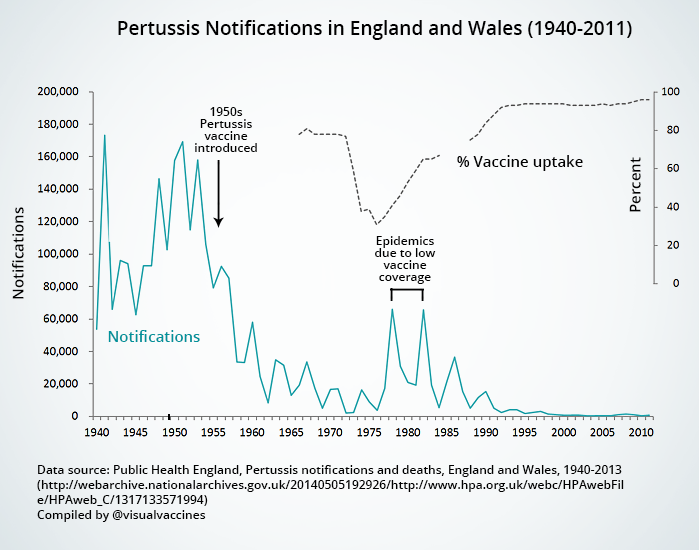
\includegraphics[height=0.7\linewidth]{ukpertussis}
  \caption{Pertussis Notifications in England \break
  and Wales 1940-2011}  
  \label{fig:test1}
  
\end{minipage}%
\begin{minipage}{.4\textwidth}
  \centering
  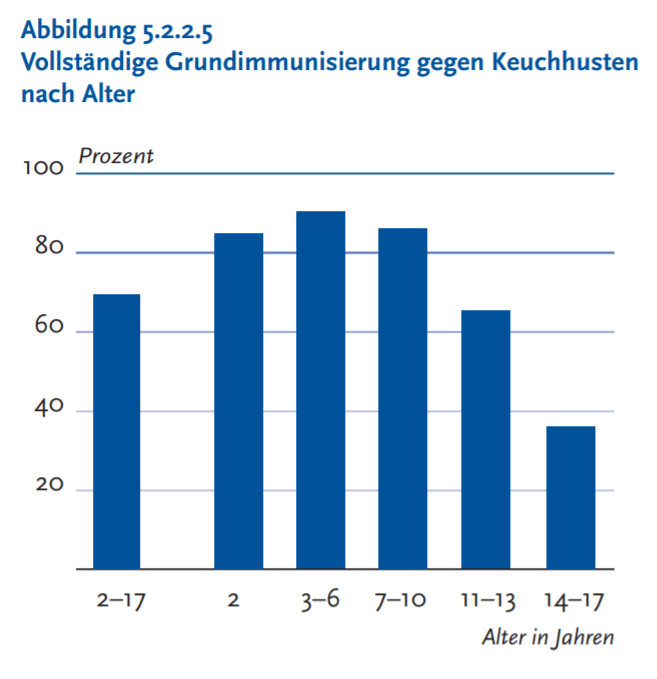
\includegraphics[height=1\linewidth]{grundimmodeutschlandpertussis}
  \caption{Basic immunisation against Pertussis by age-groups}
  \label{fig:test2}
 
\end{minipage}%
\end{figure}

Figures 1 and 2 show interesting data from two countries with good vaccination coverage, the UK and Germany. In the second the basic immunisation (having had the two first pertussis shots) of children by age-group. \footnote{Robert-Koch-Institut und BZgA: Zur Gesundheit von Kindern und Jugendlichen in Deutschland}



\section{Description of the Model}

\subsection{SIR Model}

We used an SIR model for the simulation of the spreading of Pertussis. Pertussis is transmitted by respiratory droplets human-to-human with an incubation period ranging from 9 to 14 days, while symptoms can last up to 6 weeks. \footnote{Torres Codeço, C; Mendes Luz, P; Is pertussis actually reemerging? Insights from an individual-based model, Cad. Saúde Pública vol.17 no.3 Rio de Janeiro May/June 2001}

\begin{lstlisting}
#probability of infection from outside sources
prob_for_diseases = 0.001 
prob_for_contact_infection = 0.5
\end{lstlisting}

This estimation is taken from a simulation which assesses the susceptibility of family members. We assume that a person has frequent contact with close family members and modulate the outcome with another variable that uses the probability that you meet with someone from your network on a given day to depict a realistic depiction of the society. 
\footnote{Estimation of Household Transmission Rates of Pertussis and the Effect of Cocooning Vaccination Strategies on Infant Pertussis Epidemiology 23(6):852-860, November 2012}
\vspace{14px}



\subsubsection{Modelling immunisation}
We assume that the vaccination provides 100\% safety, equal to having recovered from the disease. However, as recent research has shown that the protection considerably decreases about 10  years after the initial protection. 
To simplify the length of the protection acquired either by being vaccinated or by having recovered from Pertussis, we give people the option to vaccinate again after 8 years. The average duration of protection is 12 years with a standard deviation of 2 years, which is on the conservative side, given that only 10\% of those vaccinated are still protected 12 years after the vaccination. There is less data available to assess the immunity after having recovered from the disease, but it can be assumed to be similar to the immunity acquired by vaccination. In addition we analyse a society with a high rate of coverage, so that the majority will have acquired their immunity by vaccination.\footnote{Wendelboe, Van, Salmaso, Englund: Duration of immunity against pertussis after natural infection or vaccination. S58–S61} 
As this dynamics of waning immunity already provides us with a constant population, we do not model births and deaths, as Pertussis is not a disease that frequenly causes death. 

\subsection{Network}

The main model of our project uses a complex network representing the contacts of each person. The vertices are the individuals in the simulation and each edge is a contact between the two people. We worked with undirected networks in all our simulations. The transmission of a disease, at least in the case of pertussis, occurs if and only if the two individuals have direct contact. Meaning if Person A has contact to Person B, then Person B has automatically also contact to Person A. That context is better represented by an undirected network. However, our simulation works for directed networks as well.
All networks we used were also connected, which means that there is a path between each two vertices. All social networks nowadays are that way, in particular small sized systems like in our simulation. Moreover, unconnected individuals do not play a role as the disease can only be transmitted by human contact.
\vspace{14px}

\begin{figure}
\centering
\begin{minipage}{.5\textwidth}
  \centering
  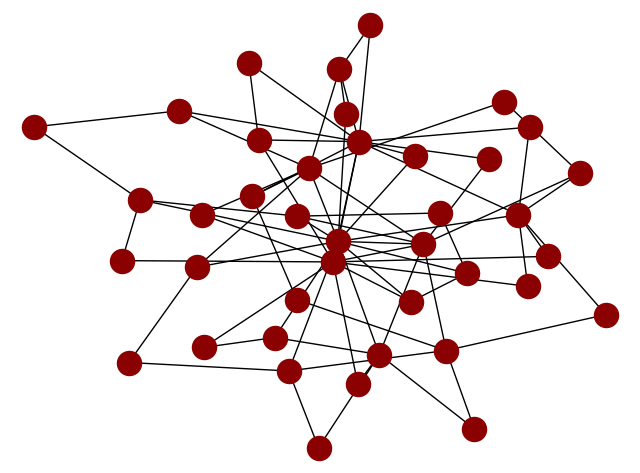
\includegraphics[width=1\linewidth]{networkplot}
  \caption{Network structure}  
  \label{fig:test3}
  
\end{minipage}%
\begin{minipage}{.5\textwidth}
  \centering
  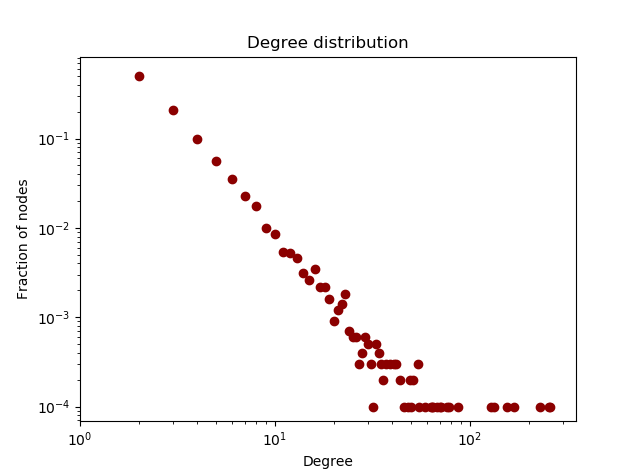
\includegraphics[width=1\linewidth]{degreedistribution}
  \caption{Degree distributions}
  \label{fig:test4}
 
\end{minipage}%
\end{figure}

As studied by Barabasi, randomly generated graphs are not a good representation of real human networks as some people will have contact to many more people than average, while most will have contact to far fewer individuals.\footnote{INSERT REFERENCE BARABASI} That is because people with a large number of contacts are more likely to connect with even more people. That means real human networks exhibit so called scale-free behavior, meaning that the degree distribution falls by some polynomial rather than being constant like in a completely random network. The Barabasi-Albert-Network reaches that by sequentially adding single nodes each with two new edges connecting randomly, but with a preference to nodes with a higher degree, to the already existing nodes. Using that process, a degree distribution of $k^{-3}$ is reached. We did create our own generator which builds a network after the Barabasi-Albert-Model. However, due to considerable runtime length we used the Barabasi-Albert-Generator from the Python Module Networkx for most of our simulation, especially for those with a high number of vertices.
\vspace{14px}


\subsection{Vaccination decision}

We assume that every person is a rational decision maker. To evaluate the probability of a person to get vaccinated, we use a static model in which each individual assesses their personal cost of getting vaccinated versus getting infected.  \footnote{INSERT RESEACH ABOUT 12 YEARS HERE}  The main parameters guiding their decision are the perceived risk of side effects of the vaccination r\_v, and perceived risk of the loss they would incur by getting the disease r\_i.

These two parameters are influenced by various factors. The statistic risks will for sure play into them, but so does the risk that an individual perceives through media statements and
the infection of people in their network, as well as influences from friends and family. Financial costs are likewise taken into consideration, be it the actual monetary cost of the vaccination or the foregone income when a person is infected and cannot work for a certain number of days. Furthermore we will assume that the disease can only be transmitted by humans. Childhood diseases like pertussis or measles are of that kind. 
The probability to get infected PI\_i is primarily determined by the proportion of people that are currently infected l\_i and the proportion of people that are vaccinated l\_c


\subsubsection{Perceived vaccination cost} 
As we consider the ratio of the perceived cost of vaccination and the perceived cost of infection (i.e. getting sick) and not the absolute values, we set the perceived cost of vaccination arbitrarily to 1 at the start. This number does not only include the monetary cost, but also the risk of side effects and other factors, which we do not consider separately. For finding the perceived cost of infection, we go back to our initial assumption that a voluntary vaccination policy is in place. That means that the initial perceived cost of infection is related to the initial coverage level in our system. If initially 97\% of the people are vaccinated, we set the perceived vaccination cost in such a way that the expected gain due to vaccination is slightly negative for every person exceeding the 97\% coverage level.

\begin{equation}
E(P,p) = -rP +(1-P)*i
\end{equation}


expected\_gain = - perceived risk of vaccination + infection cost *(infection level * (1 - coverage level)* risk of infection) 

\vspace{14px}


\subsubsection{Perceived infection cost}
The perceived vaccination cost of a person changes in two scenarios:

1. When someone in the immediate surroundings is infected, the perceived infection cost rises by a factor of 1.2 (after recovery of the contact it decreases by 0.9).

2. When the global level of 

\subsection{One person among N people}
To illustrate this, let us have a look how a person A takes the decision to vaccinate: 
We initialise each person with a value for perceived vaccination cost and perceived infection cost (which are the same for everyone at the beginning. 
If a person B in the network of A falls ill, A's perceived infection cost rises by a factor of 1.2. If another person C in A's network were to fall ill, A's perceived infection cost would rise by a factor of 1.2 again. After person B recovers, A's perceived infection cost are multiplied by a factor of 0.9, the same is true when person C recovers, leaving person A with a perceived risk of infection of 1.1664 compared to 1 at the beginning, accounting for the fact that the person is more aware of the cost of the disease because B and C in their network have been affected. 

\subsection{Equilibria for N people}
In addition to the "local" information of the nodes in the network of the person, there is also information on the general coverage and infection level in society available to the individual, as well as an additional factor that we call 


\section{Implementation}
The model was implemented using Python. First, we wrote the basic SIR model with infection and recovery. Then we added the "vaccination function" which returns whether a person is getting vaccinated or not. 

\vspace{14px}

\subsection{General Principle of the Simulation}
The programme has an object-oriented approach, meaning that the main program is executed by objects of a class Person in vacc.py. Each Person is one individual in our model. There are two derived classes, each corresponding to a way of simulating the interactions between those individuals:
\vspace{14px}

\textbf{Grid\_Person:} Places people on a two-dimensional plane, where each pixel stands for one Person. Not a very realistic model, but it allows for nice graphical representations and animations.
\vspace{14px}

\textbf{Network\_Person:} More realistic and thus the one used for the whole analysis. Every Network\_Person has an adjacency list of all its contacts and can only interact with those.
\vspace{14px}

Each timestep (one day) several member functions are called to refresh the status of each Person.

\textbf{Next\_day():} Checks, whether immunisation or infection is still active or refreshes the corresponding variables if this is not the case

\textbf{Get\_vaccinated():} Every day, each person decides whether to get vaccinated today, depening on the expected gain for themselves. The details of that can be found in 4.3. 

\textbf{Start\_infection(probability\_to\_meet):} An infected person starts being contagious 7 days after being infected until the end of incubation time, as we expect that sick people do not mingle anymore and are only attended by those who have been vaccinated.\footnote{Bundeszentrale für Gesundheitliche Aufklärung Germany, Keuchhusten \break
$www.infektionsschutz.de/erregersteckbriefe/keuchhusten/\#c3580$, accessed 30.11.2018} The probability\_to\_meet represents the probability of two people meeting each other, with the probability of being infected is prob\_for\_contact\_infection.
\vspace{14px}


\subsection{Initialisation for long time analysis}
The main goal of the long-term analysis is to investigate if and when the disease can reemerge. To model this, a few new functions and parameters are needed. Following the assumptions about waning immunisation \textbf{(explained in 4.1.1)}, we approximate the length of immunity of an individual by a gaussian with a mean of 12 years and a standard deviation of two years. The individuals obviously do not know, whether they are still immune, but can vaccinate again after 8 years,consistent with recommendations from health organisations. 

Another parameter that we introduce is a random probability to be infected. Pertussis is only transmitted by other humans. However, that random probability is needed as the disease would die out quickly due to the small size of our system, and represents contact with others outside the system (e.g. travellers) that would otherwise not be accounted for. 

The last but arguably most important parameters are the perceived cost of vaccination and infection. As the literature on this topic is very theoretical in nature, we took and adjusted a simple game-theory based model by Heal\footnote{HEAL ............} and fit it to our model. \textbf{(Read more in 4.3.1 and 4.3.2).} The first problem is that no one vaccinates if nobody is infected. That is evidently false, so we set the infection level to a minimum of 0.1 percent, corresponding to the probability of getting infected by an outside person.
\vspace{14px}


Letting this model run yields no results, as it operates in an equilibrium. As soon as one person’s immunisation becomes inactive they will immediately vaccinate again, resulting in a constant coverage level. This is also consistent with the real situation. If 97\% of the people have decided to vaccinate and the opinion of everybody remains the same, they will immediately vaccinate again upon losing immunisation.
\vspace{14px}

\subsubsection{Vaccination scares}
That means we have to introduce a parameter to vary their opinion, which we call vaccination scares. At different times we change the perceived cost of vaccination of some proportion of the population just like a anti-vaccine newspaper article or television documentary for example would.
If there has not been a noticeable outbreak, the perceived vaccination percent of 30\% of the population (selected randomly) is increased by a factor of 1.5, this happens all 500 days at maximum. Since these dynamics are hard to model, we decided to implement it this way. However, if you were to implement this mechanism in a different way, you would get similar results, the main difference being the time intervals at which those events occur. Since we are not trying to predict when an outbreak will occur, we are indifferent to the exact timing and instead observe the reaction of the system to such a vaccination scare. 




\section{Simulation Results and Discussion}


\subsection{Initial breakout}

\begin{figure}
\begin{center}
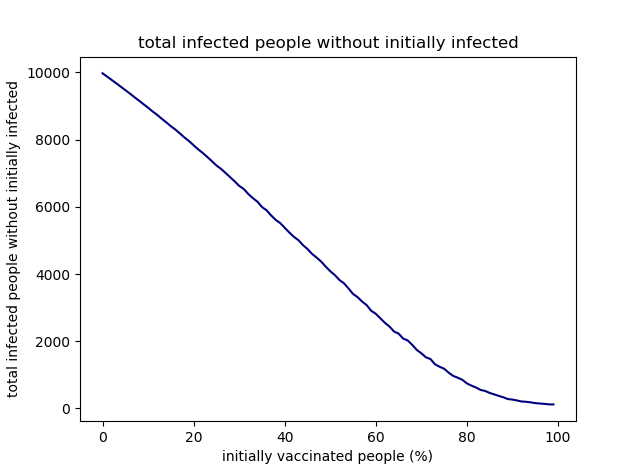
\includegraphics[scale=0.5]{totalinfecwoinitinfec}
\end{center}
\caption{caption}
\label{fig:test5}
\end{figure}
total infected people without initially infected

In our first test, we ran our model with different levels of initial coverage level, analogous to the study by Hein on Herd Immunity.\footnote{Fine, Paul, Ken Eames, and David L. Heymann. "“Herd immunity”: a rough guide." Clinical infectious diseases 52.7 (2011): 911-916.} As predicted by other models, our results indicate that there is a threshold of vaccination coverage, which is needed to keep the number of infections low. On the x-Axis we have the percentage of initially vaccinated people (we do not take into account waning immunity as we only run the programme for a period of 500 days), on the y-Axis the absolute number of people who get infected at some point during this time period, excluding the persons who are infected at the start of the simulation (just one person in our case). It is important to note that we generate figure 3 by running the programme 50 times for each initial vaccination level and taking the average, hence the smooth curve. The standard deviations were as following: 21,25260693
 total infected people without initially infected

This also coincides with the Vaccination coverage $V_{c}$ and the Basic Reproduction Number $R_{c}$ of Pertussis, our model yields -----------------------------------------------------------------------------------------------------------------------. (This is based on the standard SIR model, which in our case was slightly modified). 

\begin{equation}
V_{c} = 1-\dfrac{1}{R_{0}}
\end{equation}

The Basic Reporduction Number indicates the number of cases that one single case generates over the period in which the patient is contagious. The range of this measeure for Polio is wide, ranging from 5 to 18 in the literature. When comparing the output of our model (threshold where no new cases occur) and calculate the Basic Reproduction Number, we get 12, which is well within the range of observed BRNs, and makes sense, taking into account that we account for the number of contacts in other parameters.\footnote{McGirr, Estimation of the underlying burden of pertussis in adolescents and adults in Southern Ontario, Canada} 




\subsection{Long-term study}
As explained in 5.2.1, we introduced vaccination scares in our long-term model, which results in a system that is a lot more unstable than the initial model without such supplement. Not only is this expected, it is also realistic to assume that outbreaks happen randomly and are not 'scheduled'. 

We ran simulations for 7000 days for the long-term study. As mentioned before, due to the large number of random parameters, outbreaks happened at different periods in time, but they always looked similar, as can be seen in figure 4 and in a close-up in figure 5. As immunity is waning and the level of infection is low for a long period, the parameters determining vaccination in many people do not cross the threshold where they get vaccinated. This gives the disease a window where a seizable portion of people are not protected, resulting in an outbreak of the disease. When we look at the number of infections in these simulations, we talk about 60 cases in a population of 5493\footnote{project90.tsv (5493 vertices): https://opr.princeton.edu/archive/p90/}. When comparing  this to numbers of outbreaks in German federal countries, we see that the \footnote{DEUTSCHE BUNDESLÄNDER}


\begin{figure}
\centering
\begin{minipage}{.5\textwidth}
  \centering
  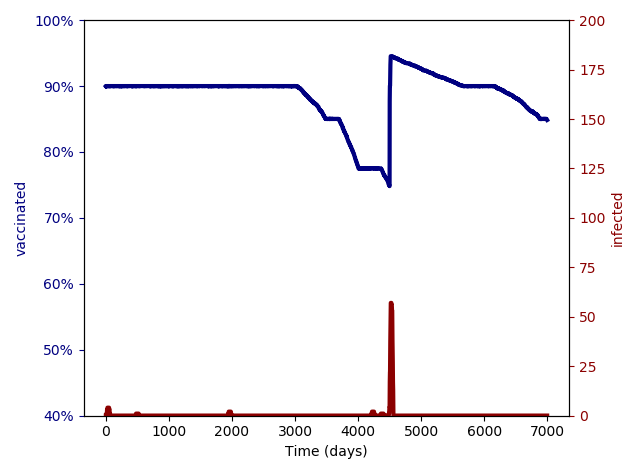
\includegraphics[width=1\linewidth]{02aedges200001p2fixedtime5001p5sv0p001}
  \caption{graph 1}  
  \label{fig:test6}
  
\end{minipage}%
\begin{minipage}{.5\textwidth}
  \centering
  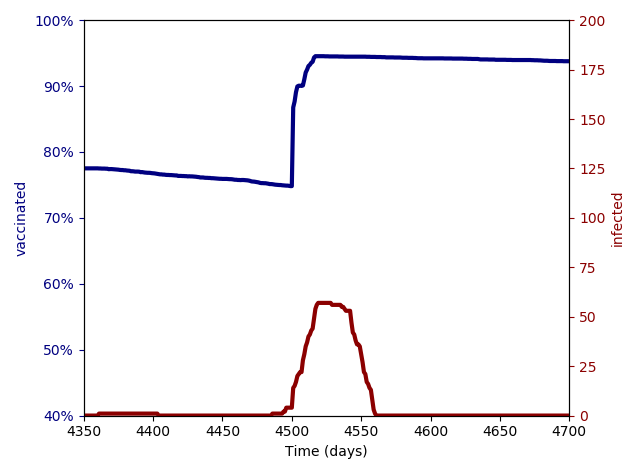
\includegraphics[width=1\linewidth]{02bedges200001p2fixedtime5001p5sv0p001}
  \caption{graph 2}
  \label{fig:test7}
 
\end{minipage}%
\end{figure}



\subsection{Limitations}
As with any model, this model has a range of limitations that result from the simplifying assumption that were taken.

The short term analysis has the same limitations as a standard stochastic SIR model. All the parameters of the disease like incubation time or the probability of transmission are the same for every person. However, having the stochastic SIR on the network approximates the transmission of the disease already much better than a deterministic SIR.

In the long term analysis people decide if they should get vaccinated based on perfect information of infections of other people. That is the same as Bauch did it in his deterministic model. In contrast to that, our model has two dynamic variables, perceived infection cost and perceived vaccination cost. As perceived vaccination cost is dependent on the contacts, our model has a “cluster effect”. This means that people who are closely connected are prone to doing the same thing as their connections, which is something we can observe in society, where those who criticise/favour vaccinations often influence their friends' decisions. Additionally we introduced vaccination scares that change the long term properties of the system. Both effects are very hard to quantify, as they are complicated and unpredictable processes. Therefore, our model simplifies these effects; this could be extended to account for more variance in reactions than we were able to account for. However, for the purpose of showing the phenomenon of declining coverage and the resurgence of diseases it is well suited. 
 

\subsection{Algorithm Performance}
As we have a stochastic model on a network performance, a fast runtime is important for scaling and running the test multiple times. For each day in our simulation we need to iterate through all people to update their status. The only operations possibly taking more than constant time are the interactions of the people. That depends on the network. If the highest number of edges for one vertice is not constant, it will prolong the runtime drastically. However, this effect was minor for all networks we tested. So for the length of the simulation d, the number of people n, and the number of edges m, the simulation has a time complexity of O(d*n*m). Therefore, we expect a linear dependence of people and the other way around for a constant number of days (assuming m is constant in n). The graphs show exactly that dependence. \footnote{INSERT TIMO'S GRAPH HERE}

\section{Summary and Outlook}
We found the critical coverage level which needs to be reached or surpassed in order to prevent an outbreak, with several 

\section{References}
Table of References: 
\vspace{14px}

Bauch, C. T., \& Earn, D. J. (2004). Vaccination and the theory of games. Proceedings of the National Academy of Sciences, 101(36), 13391-13394.
\vspace{14px}

Office of Population Research, Princton University: https://opr.princeton.edu/archive/p90/

Caldarelli, Guido, and Alessandro Chessa. Data science and complex networks: real case studies with Python. Oxford University Press, 2016.

Coolen, Anthony CC, Alessia Annibale, and Ekaterina Roberts. Generating random networks and graphs. Oxford University Press, 2017.

Eshel, I. (1996). On the changing concept of evolutionary population stability as a reflection of a changing point of view in the quantitative theory of evolution. Journal of mathematical biology, 34(5-6), 485-510.
\vspace{14px}

Fine, Paul, Ken Eames, and David L. Heymann. "“Herd immunity”: a rough guide." Clinical infectious diseases 52.7 (2011): 911-916.
\vspace{14px}

Heal, G., \& Kunreuther, H. (2005). The vaccination game. Risk Management and Decision Processes Center Working Paper, (05-10). 
\vspace{14px}

McGirr, Ashleigh A et al. “Estimation of the underlying burden of pertussis in adolescents and adults in Southern Ontario, Canada” PloS one vol. 8,12 e83850. 23 Dec. 2013, doi:10.1371/journal.pone.0083850
\vspace{14px}

Estimation of Household Transmission Rates of Pertussis and the Effect of Cocooning Vaccination Strategies on Infant Pertussis Epidemiology 23(6):852-860, November 2012
\vspace{14px}

Robert-Koch-Institut und BZgA: Zur Gesundheit von Kindern und Jugendlichen in Deutschland, ISBN 978-3-89606-109-7, 05.05.09

Wendelboe AM, Van RA, Salmaso S, Englund JA: Duration of immunity against pertussis after natural infection or vaccination. Pediatr Infect Dis J 2005; 24(5 Suppl): S58–S61
\vspace{14px}

Torres Codeço, C; Mendes Luz, P; Is pertussis actually reemerging? Insights from an individual-based model, Cad. Saúde Pública vol.17 no.3 Rio de Janeiro May/June 2001
\vspace{14px}

$https://ourworldindata.org/vaccination$ 
\vspace{14px}

$https://www.gapminder.org/data/$ search for 'vaccine'
\vspace{14px}

Immunization coverage, system indicators and schedule, and disease incidence $www.who.int/immunization/monitoring_surveillance/data/en$


\newpage




\end{document}  



 
